\documentclass[authordate, empirical]{jote-new-article}


\usepackage{balance}
\jotetitle{Smile, You’re on Camera: Investigating the Relationship between Selfie Smiles and Distress}
\keywordsabstract{mobile sensing, video, selfie, facial expression, smile}
\abstracttext{Background: This study examined the relationship between (1) participant smiling in daily “selfie” videos and (2) self-reported distress. Given the extensive use of digital devices for sharing expressions of non-verbal behavior, and some speculation that these expressions may reveal psychological states—including emotional distress—we wanted to understand whether facial expression in these TikTok-like videos were correlated with standardized measures of psychological distress. Based on the work of Paul Ekman and others, which posits that facial expressions are universal reflections of people’s inner states, we predicted that smiling would be inversely related to psychological distress.
Method: Twenty-four undergraduate students, aged 18+ years \textit{(M = 18.35, SD = 2.75)}, were prompted to record a two-minute selfie video each evening during two weeks of data collection (i.e., 14 total days). They were instructed to describe various aspects of their day. They also completed self-report questionnaires at the end of each assessment week, including the Depression Anxiety Stress Scale (DASS), Perceived Stress Scale (PSS), and the Pittsburgh Sleep Quality Index (PSQI).
Results: A counterintuitive effect was observed whereby smiling intensity during selfie videos was positively correlated with individual differences in anxiety, depression, and stress.
Discussion: This study challenges the common view that facial expressions necessarily reflect our inner emotions. It provides preliminary evidence that a mobile sensing app that captures selfies—along with other naturalistic data—may help elucidate the relationship between facial expressions and emotions.}
\runningauthor{Lind et al.}
\jname{Journal of Trial \& Error}
\jyear{2024}
\paperdoi{10.36850/8716-5abe}
\paperreceived{March 3, 2022}
\author[1]{\mbox{Monika Lind\orcid{0000-0001-5634-2470}}}
\affil[1]{Department of Psychology; University of Oregon; USA Department of Psychological Science; School of Social Ecology; University of California, Irvine; USA}
\corremail{\href{mailto:m.lind@uci.edu}{m.lind@uci.edu}}
\corraddress{UC Irvine}
\runningauthor{Lind et al.}
\author[2]{\mbox{Michelle Byrne\orcid{0000-0002-4180-8095}}}
\affil[2]{University of Oregon; USA School of Psychological Sciences; Turner Institute for Brain and Mental Health; Monash University; Australia}
\author[3, \textdagger]{\mbox{Sean Devine\orcid{0000-0002-0445-2763}}}
\affil[3]{Department of Psychology; McGill University; Canada}
\author[4]{\mbox{Nicholas Allen\orcid{0000-0002-1086-6639}}}
\affil[4]{Department of Psychology; University of Oregon; USA}
\paperaccepted{March 6, 2024}
\paperpublished{May 24, 2024}
\paperpublisheddate{2024-05-24}
\jwebsite{https://journal.trialanderror.org}

\begin{document}
\begin{frontmatter}
  \maketitle
  \begin{abstract}
    \printabstracttext
  \end{abstract}
\end{frontmatter}




























\lettrine{T}{his} is a small study with counterintuitive findings that bear on our understanding of facial expressions and our use of selfie data. This study lands on the growing stack of publications that support the view that facial expressions are something other than an accurate readout of a person's internal state (Barrett et al., 2019). Furthermore, this study shows that a special aspect of our lab's mobile sensing app, the ability to collect \emph{TikTok}-like “selfie” videos, may provide meaningful insights into psychological states.\customfootnote[\textdagger]{During the peer review process Sean Devine peer reviewed the article and signed his review, in which he pointed out that the pre-planned analysis was not the most efficient use of the data, given the data’s nested structure. Devine provided multiple alternatives for how to model the data. The authors subsequently contacted Devine to join as an author. After this occured and changes were made to the article, the article again went through independent peer review.}



This study draws its data from the Effortless Assessment of Stressful Experiences project, a small but mighty pilot. The project aimed to find out whether a mobile sensing app, the Effortless Assessment Research System (EARS; Figure 1), could produce meaningful data about distress without EARS itself driving research participants crazy. This study builds on two existing publications from the project: a paper introducing EARS, including information about its excellent acceptability (Lind et al., 2018), and a paper on the associations between EARS data (typed text), self-reported stress, and biological markers of inflammation (Byrne et al., 2021).



\begin{takeHomeMessage}

  This is a small study with counterintuitive findings. It further loosens the grip of the common view that our facial expressions necessarily reflect our inner emotional states, and it provides preliminary evidence that a mobile sensing app that captures selfies can help elucidate the relationship between facial expressions and emotions.

\end{takeHomeMessage}





\begin{figure}[b]
  \begin{fullwidth}
    \centering
    
\includegraphics[width=.5\linewidth]{media/image1.png}

    \caption{EARS app icon.}
  \end{fullwidth}

  \label{fig:rId8}



\end{figure}


\begin{figure}[b!]
  \begin{fullwidth}
    \centering
    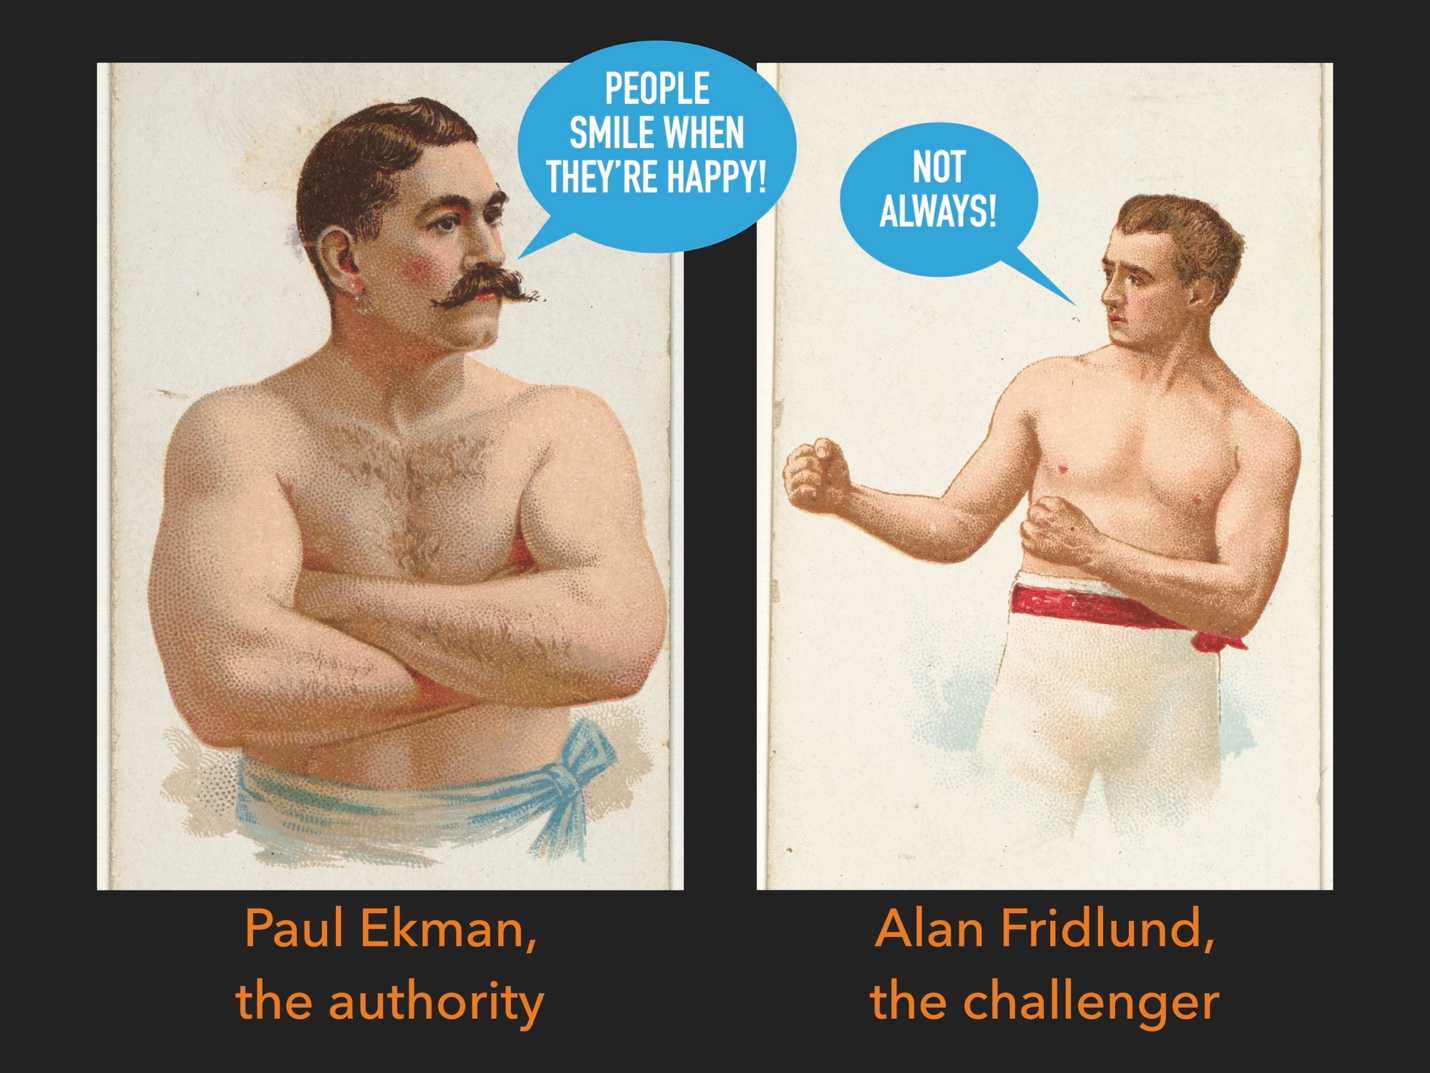
\includegraphics[width=.8\linewidth]{media/image2.jpeg}

    \caption{Dr. Ekman and Dr. Fridlund; images from the public domain.}
  \end{fullwidth}

  \label{fig:rId9}


\end{figure}

This study focuses on the relationship between (1) participant smiling in selfie videos captured by EARS and (2) self-reported distress. The field of facial expression research is rich with nuanced research and theories that defy distillation…but that won't stop me from trying! Paul Ekman advanced the expressed emotion framework for facial expressions, which posited that facial expressions are universal reflections of people's inner states (Ekman, 1993; Ekman \& Friesen, 1971). In a classic academic plot twist, Alan Fridlund, Dr. Ekman's junior collaborator, contradicted his thesis (Figure 2). Dr. Fridlund took a behavioral ecology view of facial expressions that posited that facial expressions primarily serve a person's communication goals and therefore may not always align with their inner emotions (Fridlund, 1994).



This debate continues to animate facial expression research specifically and emotion research more broadly (Ekman, 2016). Fridlund's behavioral ecology view of facial expressions leads a robust field of research advancing motivation-communication views, while Lisa Feldman Barrett has led the development of constructivist emotion theories, which characterize emotion and facial expressions as comprised of orthogonal dimensions of valence and arousal (Barrett, 2006; Mayo \& Heilig, 2019). A growing wave of evidence undermines Ekman's framework, including studies conducted in the same settings where Ekman first found support for his views (i.e., in small, indigenous societies; Crivelli et al., 2017; Gendron et al., 2018). This wave has a sturdy bulwark to overcome: In a survey of about 150 top researchers of emotion, 80\% of respondents endorsed an Ekman-aligned view that facial expressions provide universally interpretable read-outs of emotions (Ekman, 2016).



Current research on selfies tends to focus on publicly available images, e.g., images on Instagram. Deeb-Swihart and colleagues (2017) used computer vision and network analysis techniques on 2.5 million selfies from Instagram, the largest empirical analysis of selfies at the time. They categorized the selfies into typologies of identity statements and found that the categories present in online selfies reflect the same categories present in real-life identity statements (e.g., wealth, health, and physical attractiveness). This focus on the identity-related content of selfies typifies current selfie research. Psychological studies of facial expressions in selfie images and videos tend to focus on the degree to which human judgment and machine learning approaches can accurately perceive the personality traits of the selfie subjects (Kachur et al., 2020; Qiu et al., 2015). Meanwhile, medical studies of facial expressions in selfies have produced promising findings related to the detection of illnesses that affect the expressiveness of the face, e.g., Parkinson's Disease (Grammatikopoulou et al., 2019). We believe this is the first study to focus on the relationship between facial expressions in selfie videos and psychological distress.



Valuing the simplicity of the expressed emotion framework and recognizing it as the default view in the field, we decided to align our hypotheses with Ekman. We hypothesized that within-subject increases in self-reported distress would be associated with decreases in smiling intensity.












\begin{figure}[t]
  \begin{fullwidth}
    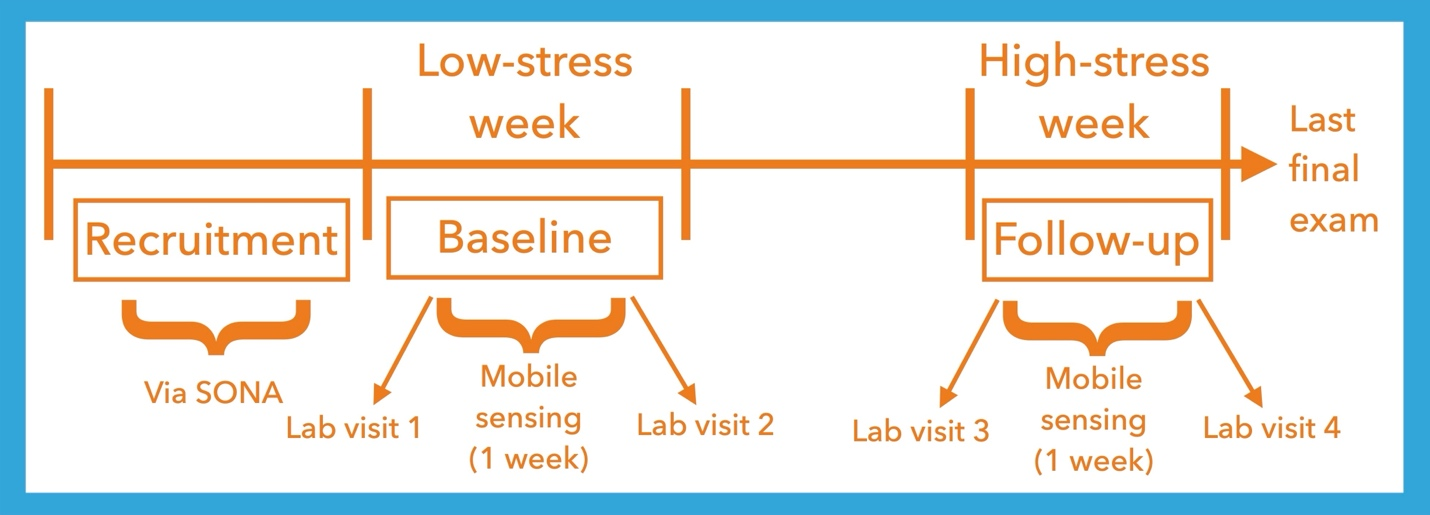
\includegraphics[width=\linewidth]{media/image3.jpeg}

    \caption{Timeline of the EASE study.}
  \end{fullwidth}

  \label{fig:rId10}


\end{figure}





\section{Method}







\subsection{Protocol}



We used an academic stress paradigm to test this hypothesis (Figure 3). The academic stress paradigm takes advantage of the varying degrees of stress built into each academic term (Zunhammer et al., 2013). In our case, the academic stress paradigm let us gather mobile sensing and questionnaire data twice: once during a low-stress week (nothing major due) and once during a high-stress week (finals week). We determined the specific data-gathering schedule for each participant based on the participant's report of their major assignment deadlines and their last final exam. (If you, dear reader, are on the quarter system and you're thinking, “There are no low-stress weeks!” \emph{ahem}, hang onto that thought.)
















\subsection{Participants}



Undergraduates at a large public university in the American Northwest enrolled in the study via the Psychology and Linguistics human subjects pool during the 2016-17 academic year. Inclusion criteria were using an Android phone and not having an immunological medical condition (which was related to a study aim not reported in this paper). All participants used Android phones because this classic 2016 vintage of EARS only worked on Android. During the study period, reports indicated that Android users comprised at least half of the American smart phone market (Comscore, 2016; Siegal, 2017). A contemporaneous study showed that there was little empirical support for personality differences between Android and iOS users at that time (Götz et al., 2017). Additional contemporaneous research on the characteristics of iPhone versus Android users is lacking. As such, a pilot study with only Android users is reasonable. Participants received \$50 compensation. The university's Institutional Review Board approved the study (protocol number 07212016.019), and participants provided informed consent during the first lab visit.



Participants were 25 undergraduate students, aged 18+ years (\emph{M} = 18.35, \emph{SD} = 2.75). Twenty-four participants completed the whole study. Twelve participants (50\%) were cisgender female, and 12 (50\%) were cisgender male; 12\% were Asian, 64\% Caucasian, 12\% Hispanic, and 12\% Multiracial. The yearly income of participants' parents ranged from lower to upper-middle class (\emph{M} = \$88,625.00, \emph{SD} = 62,009.69).







\subsection{Measures}



To collect facial expression data, EARS prompted each participant to record a two-minute selfie video each evening during data collection (14 total days). In each selfie video, we instructed participants to state their name, date, time, and the weather. We then prompted them to describe one thing that happened that day that was positive (“What was the best thing that happened today, and can you describe it?”), and one thing that was negative (“What was the most difficult thing that happened today, and can you describe it?”).



As part of the battery of self-report questionnaires at the end of each assessment week, participants completed the Depression Anxiety Stress Scales (DASS), Perceived Stress Scale (PSS), and the Pittsburgh Sleep Quality Index (PSQI). The DASS is a 42-item questionnaire designed to measure the three related negative emotional states of depression, anxiety, and tension/stress (Lovibond \& Lovibond, 1995). This version of the DASS has high internal consistency across clinical and community samples (Antony et al., 1998). The PSS is a 14-item questionnaire designed to measure perceived stress (Cohen et al., 1983). This version of the PSS has Cronbach's alpha values consistently over 0.70 across multiple cultures and countries (Lee, 2012). The PSQI measures subjective sleep quality and quantity (Buysse et al., 1989). For the DASS, PSS, and PSQI, we instructed participants to respond based on their experiences over the last week.



At baseline, participants completed the computerized version of the Stress and Adversity Inventory (STRAIN), an NIMH/RDoC-recommended instrument for measuring cumulative exposure to life stress (see \url{https://www.strainsetup.com/}; Slavich \& Shields, 2018). The STRAIN uses intelligent logic to shape the interview based on the participant's responses.






\subsection{Data Analysis}



\begin{table*}[b]
  \begin{fullwidth}
    \caption{Means, standard deviations, and ranges of smiling intensity, DASS subscales (Depression, Anxiety, Stress), perceived stress (PSS), and self-reported sleep quantity in hours (PSQI) by week, plus the change in the means across weeks.}
    \begin{tabularx}{\linewidth}{@{} X r l l r l l l @{}}
      \toprule
               & \multicolumn{3}{c}{\textbf{Low-Stress Week}} & \multicolumn{3}{c}{\textbf{High-Stress Week}}
               & \textbf{Change}                                                                                                                                      \\


               & Mean                                         & \textit{SD}                                   & Range      & Mean  & \textit{SD} & Range      &       \\
      \midrule

      Smiling  & 0.60                                         & 0.44                                          & 0.02-1.60  & 0.55  & 0.43        & 0.02-1.65  & -0.05 \\

      DASS-Dep & 7.42                                         & 6.88                                          & 0.00-23.00 & 6.46  & 5.51        & 0.00-23.00 & -0.96 \\

      DASS-Anx & 5.46                                         & 5.00                                          & 0.00-17.00 & 7.67  & 5.54        & 0.00-21.00 & +2.21 \\

      DASS-Str & 11.00                                        & 8.24                                          & 0.00-26.00 & 12.84 & 9.06        & 1.00-33.00 & +1.84
      \\

      PSS      & 24.57                                        & 8.50                                          & 6.00-37.00 & 25.04 & 10.05       & 4.00-40.00 & +0.47 \\

      Sleep    & 6.78                                         & 1.30                                          & 4.00-9.00  & 6.98  & 1.52        & 2.00-9.00  & +0.20 \\
      \bottomrule
    \end{tabularx}
  \end{fullwidth}
\end{table*}

The 24 participants generated 325 selfie videos. We used OpenFace, a “facial behavior analysis toolkit,” to conduct automated analysis of participants' smiles. OpenFace output includes facial landmark detection, facial landmark and head pose tracking, facial action unit recognition, gaze tracking, and facial feature extraction (Baltrusaitis et al., 2018). Action units (AUs) refer to small movements of the face, like action unit 6 (“the cheek raiser”) or action unit 9 (“the nose wrinkler”). We focused on facial action unit 12 (AU12), commonly referred to as the “lip corner puller,” which captures smiling. Smiling warrants special attention for two reasons: One, the smile is the most common facial expression in the datasets used to develop facial expression analysis software, so it is the facial expression that OpenFace detects most reliably; and two, smiling is meaningful around the world and relates to important life outcomes (Godoy et al., 2005). OpenFace produces both a categorical present/absent measure of action units and a continuous intensity measure of action units. We focused on the intensity measure (range: 0-5) to capture nuance in smiling behavior beyond just presence and absence. We chose not to check the content of the selfie videos because we wanted to determine whether fully automated facial expression analysis (i.e., without a human in the loop), was a viable approach for future, large-scale studies.




\begin{table}[t]
  \begin{fullwidth}
    \caption{Multilevel model regressing smiling intensity nested within participant on standardized change scores of DASS subscales and sleep crossed with week.}
    \begin{tabularx}{\linewidth}{@{} l r r r @{}}
      \toprule
      \textbf{Predictor}       & \textbf{Estimate} & \textbf{95\% CI} & \textbf{\emph{p}-value} \\
      \midrule

      (Intercept)              & -0.02             & -0.36 – 0.33     & 0.922                   \\

      Week                     & -0.08             & -0.27 – 0.11     & 0.399                   \\

      Anxiety change           & -0.08             & -0.71 – 0.55     & 0.807                   \\

      Depression change        & -0.23             & -0.69 – 0.23     & 0.332                   \\

      Stress change            & -0.01             & -0.55 – 0.53     & 0.971                   \\

      Sleep change             & 0.18              & -0.16 – 0.52     & 0.292                   \\

      Week x Anxiety change    & 0.08              & -0.26 – 0.42     & 0.642                   \\

      Week x Depression change & 0.01              & -0.24 – 0.26     & 0.929                   \\

      Week x Stress change     & 0.05              & -0.24 – 0.35     & 0.719                   \\

      Week x Sleep change      & -0.08             & -0.28 – 0.11     & 0.410                   \\
      \midrule

      \multicolumn{4}{@{}l@{}}{Marginal \emph{R}\textsuperscript{2}: 0.117}                     \\
      \multicolumn{4}{@{}l@{}}{Conditional \emph{R}\textsuperscript{2}: 0.747}
      \\
      \bottomrule
    \end{tabularx}
  \end{fullwidth}
\end{table}

\begin{table}[th!]
  \begin{fullwidth}

    \caption{Mean and standard deviation of smiling intensity by gender.}
    \begin{tabularx}{\linewidth}{@{} X l l @{}}
      \toprule
      \textbf{Gender}  & \textbf{\emph{N}} & \textbf{Smiling Intensity} \\
      \midrule

      Cisgender Female & 12                & 0.68 (\textit{SD} = 0.46)  \\

      Cisgender Male   & 12                & 0.47 (\textit{SD} = 0.34)  \\
      \bottomrule
    \end{tabularx}


    \vspace*{2\baselineskip}
    \caption{Mean and standard deviation of smiling intensity by racial and ethnic identity.}
    \begin{tabularx}{\linewidth}{@{} X r l @{}}
      \toprule
      \textbf{Race/Ethnicity} & \textbf{\textit{N}} & \textbf{Smiling Intensity} \\
      \midrule


      Asian                   & 3                   & 0.61 (\textit{SD} = 0.38)  \\

      Hispanic                & 3                   & 0.21 (\textit{SD} = 0.17)  \\

      Multiracial             & 3                   & 0.45 (\textit{SD} = 0.31)  \\

      White                   & 15                  & 0.67 (\textit{SD} = 0.44)  \\
      \bottomrule
    \end{tabularx}
  \end{fullwidth}
\end{table}


To test our hypothesis that smiling intensity would decrease as distress increased, we planned to leverage our within-subjects design to test whether change in smiling during selfie videos between the low-stress week (Time 1) and the high-stress week (Time 2) would predict change in self-reported symptoms over the same assessment periods. (Because we did not have daily questionnaire scores, we were unable to test the association of daily smiling with daily distress.) Our plan entailed calculating Time 1 and Time 2 averages for smiling and questionnaires, regressing Time 2 scores on Time 1 scores for smiling and questionnaires, then regressing the residuals of the questionnaire scores on the residuals of the smile intensity scores. Due to the small number of confirmatory hypotheses, we did not correct for multiple comparisons.

% \begin{table}[b]
%   \begin{fullwidth}
%     \caption{Mean and standard deviation of smiling intensity by racial and ethnic identity.}
%     \begin{tabularx}{\linewidth}{@{} X l l @{}}
%       \toprule
%       \textbf{Race/Ethnicity} & \textbf{\textit{N}} & \textbf{Smiling Intensity} \\
%       \midrule


%       Asian                   & 3          & 0.61 (\textit{SD} = 0.38)           \\

%       Hispanic                & 3          & 0.21 (\textit{SD} = 0.17)           \\

%       Multiracial             & 3          & 0.45 (\textit{SD} = 0.31)           \\

%       White                   & 15         & 0.67 (\textit{SD} = 0.44)           \\
%       \bottomrule
%     \end{tabularx}
%   \end{fullwidth}
% \end{table}
\section{Results}







\subsection{Hypothesis Testing}



First, we checked to see if the academic stress paradigm had the desired effect: Did participants report feeling more distressed during the high-stress week? Yes, for the most part! Second, we checked smiling behavior: Did it change in the predicted direction as well? Yes, participants smiled less—numerically but not statistically significantly, \emph{hmmm}—in the high-stress week! These patterns (Table 1) presaged well for our hypothesis that increases in distress would be associated with decreases in smiling, and we were feeling pretty clever \emph{if we do say so ourselves}. When we tested our hypothesis by regressing the residuals of the symptom scores on the residuals of the smile intensity scores, however, non-significant results rudely contradicted our cleverness. Anxiety residuals regressed on smiling residuals yielded: \emph{F}(1,22) = 1.04, \emph{p} = NS, Adjusted \emph{R}\textsuperscript{2} = 0.002.











We made a final attempt at testing our hypothesis during the peer review process. We received a thoughtful, helpful, \emph{signed }review that pointed out that our pre-planned analysis was not the most efficient use of our data, given our data's nested structure. The reviewer provided multiple alternatives for how to model our data. With the blessing of the editor, we contacted the reviewer and invited him to join the paper. The reviewer —now the third author— conducted a multilevel multiple regression with smiling intensity per video nested within participant as the outcome and change scores of self-reported distress and sleep crossed with week (low-stress vs high-stress) as the predictors (Table 2). One way to articulate this model in lay terms is, ``Does smiling decrease in high-stress weeks for a person who experienced that week as more distressing?”













Look at those p-values! They're huge! (Relatively speaking, of course— we all know p-values are not measures of magnitude.) While the direction of the simple fixed effects aligned with our hypothesis that increased distress would predict decreased smiling, we once again fell far short of statistical significance.



Our null findings forced us to reckon with an inconvenient truth: The academic stress paradigm may not have worked very well. It's true that we saw changes in the hypothesized directions, but these changes were small and only statistically significant in the case of self-reported anxiety (\emph{t}(23) = -2.14, \emph{p} < .05).








\subsection{Exploratory Analyses}



From this point forward, we conducted exploratory data analysis. Given the failure of the academic stress paradigm, we decided to treat week one and week two data as multiple measurements of the same constructs. We collapsed across the weeks, calculating averages for each participant for each variable of interest (smiling, stress, anxiety, depression, and sleep). We calculated differences in smile intensity by gender and racial and ethnic identity, but we were underpowered to test the significance of these differences (Tables 3 and 4).













We moved on to exploring the relationships among the key variables. There we were, plotting bivariate associations in the hopes of resurrecting our hypothesis, when all of a sudden:







\begin{figure}[h!]
  \begin{fullwidth}
    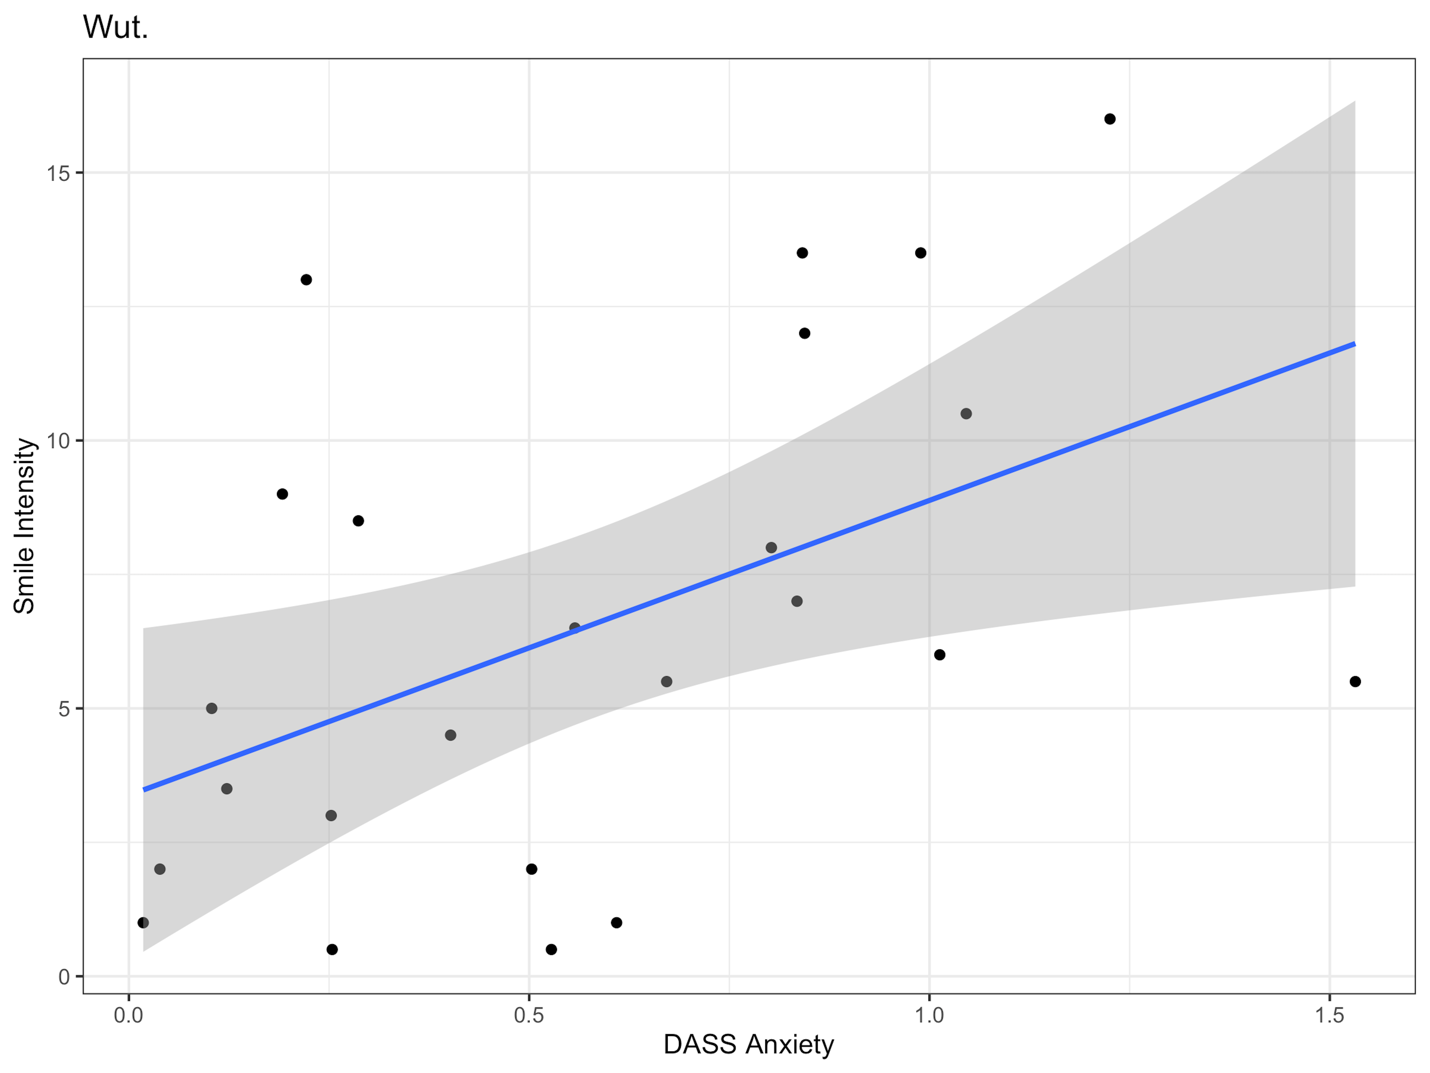
\includegraphics[width=\linewidth]{media/image4.png}

    \caption{Anxiety and smiling intensity increase together.}

  \end{fullwidth}
  \label{fig:rId11}


\end{figure}






That looks like higher anxiety is associated with… more smiling? A perusal of the correlation table fleshed out the story (Table 5).





\begin{table*}
  \begin{fullwidth}
    \caption{Pearson correlations and 95\% confidence intervals for smiling intensity, the three DASS subscales, perceived stress (PSS), lifetime stress exposure (STRAIN), and self-reported sleep quantity in hours.}
    \begin{tabularx}{\linewidth}{@{} l l l l l l l l @{}}
      \toprule
                        & \textbf{Smiling} & \textbf{DASS-Dep} & \textbf{DASS-Anx} & \textbf{DASS-Str} & \textbf{PSS}    & \textbf{STRAIN} & \textbf{Sleep} \\
      \midrule

      \textbf{Smiling}  & 1.00             & 0.38[-.03, .68]   & 0.48[.10, .74]    & 0.37[-.03, .68]   & 0.29[-.13, .62]
                        & 0.18[-.26, .56]  & -0.24[-.58, .19]                                                                                               \\

      \textbf{DASS-Dep} &                  & 1.00              & 0.52              & 0.43              & 0.45            & 0.02            & -0.20          \\

      \textbf{DASS-Anx} &                  &                   & 1.00              & 0.79              & 0.66            & 0.37            & -0.27          \\

      \textbf{DASS-Str} &                  &                   &                   & 1.00              & 0.72            & 0.36            & -0.27          \\

      \textbf{PSS}      &                  &                   &                   &                   & 1.00            & 0.27            & -0.46          \\

      \textbf{STRAIN}   &                  &                   &                   &                   &                 & 1.00            & -0.47          \\

      \textbf{Sleep}    &                  &                   &                   &                   &                 &                 & 1.00           \\
    \end{tabularx}
  \end{fullwidth}
\end{table*}






\begin{table}[b!]
  \begin{fullwidth}
    \caption{Four simple multilevel models regressing nested smiling behavior on standardized, averaged self-report measures (three DASS subscales and PSQI sleep quantity).}
    \begin{tabularx}{\linewidth}{@{} X r r  @{}}
      \toprule
      \textbf{Predictor} & \textbf{Estimate} & \textbf{95\% CI} \\
      \bottomrule

      Depression         & 0.34              & 0.02 – 0.67      \\

      Anxiety            & 0.44              & 0.13 – 0.75      \\

      Stress             & 0.35              & 0.01 – 0.68      \\


      Sleep              & -0.23             & -0.54 – 0.08     \\
      \bottomrule
    \end{tabularx}
  \end{fullwidth}
\end{table}



We set aside significance testing because of the exploratory nature of these analyses and focused instead on effect sizes. Following Cohen's (1992) guidance, we had three medium and three small effect sizes. In our data, smiling intensity had a medium, positive association with anxiety, depression, and stress; a small, positive association with perceived stress and lifetime stress; and a small, negative association with self-reported sleep quantity. In other words, smiling intensity, anxiety, depression, and stress tended to increase together.



Further investigation while accounting for multiple measurements of smiling behavior mirrored this pattern. We conducted a series of simple multilevel regressions with smiling intensity per video nested within participant as the outcome. Average depression, anxiety, stress, and sleep each took its turn as the predictor (Table 6).












While these findings may be counterintuitive, their essence—that we may smile through stress—already pervades American popular culture:







\begin{figure}[h]
  
\includegraphics[width=\linewidth]{media/image5.jpeg}

  \caption{The “This is fine” dog, from the first two panels of KC Green's comic, “On Fire,” from the series, “Gunshow” (Green, 2013); used with permission.}

  \label{fig:rId12}


\end{figure}










Do you know for sure why the dog is smiling despite the flames and smoke? We don't. The same is true of the results of this study: We know we saw an unexpected, compelling pattern in the data, and we don't know why. We'd like to offer some ways to think about these results.







\section{Discussion}







Our original hypothesis rested on the expressed emotion framework advanced by Paul Ekman, which conflicted with the behavioral ecology view of Alan Fridlund. This study, with its finding that smiling increased alongside stress, anxiety, and depression, may lend more support to Dr. Fridlund's view that facial expressions primarily serve a person's communication goals. For example, participants experiencing more anxiety might be more worried about wanting the implied audience (e.g., researchers) to like them and their videos, so they might smile more. However, we cannot say conclusively that these findings support Dr. Fridlund's view -- only that in a dichotomous scenario where Dr. Ekman and Dr. Fridlund oppose each other (such as, say, a boxing match), these findings align more with Dr. Fridlund.



The complexity of the smile as a behavioral expression could also help us think about this study's results. In facial expression research, we often use action units to describe facial configurations. To capture smiling, we measured only one facial action unit: Action Unit 12, the “lip corner puller”. Studies have found, however, that different types of smiles emerge when AU12 is combined with other action units. Dr. Ekman himself argued that there are “felt, false, and miserable smiles,” and Magdalena Rychlowska and colleagues provided a similar, more data-driven structure of three different categories of smiles: reward, affiliative, and dominance (Ekman \& Friesen, 1982; Rychlowska et al., 2017). Our simplistic index of smiling did not allow us to capture this complexity. If we were able to break the smiles down by type, we might find that one type of smile drives the association between smiling and distress.



Participants tolerated the EARS tool well, as evidenced by only one participant dropping out, zero participants needing to use the provided battery packs, and zero participants reporting interference with usual phone usage. Still, the selfie video task itself deserves some scrutiny. Each day, participants pointed their front-facing phone cameras at themselves and recorded for 30+ seconds while, in true selfie fashion, seeing themselves reflected back on their phone screens. What happens to us when we look at ourselves? How does the little Zoom box of your face affect your facial expressions during meetings? What if you're already feeling a bit stressed? Duval and Wicklund's objective self-awareness theory states that when people are made consciously aware of themselves, they compare themselves to their own standards (Duval \& Wicklund, 1972). Perhaps the reflection of participants' own faces increased their self-awareness causing them to compare themselves to their standards and smile more. This potential demand characteristic might have been exacerbated by participant anxiety and stress.



Finally, discussion of this study must take stock of the ways that it aligns with and falls short of Barrett and colleagues' recommendations in their 2019 instant classic review (Barrett et al., 2019). Our study aligns with Barrett and colleagues' calls to study facial movements in real life, combine classical psychology methods (i.e., self-report) with machine learning (i.e., automated facial analysis via OpenFace), use novel methods (i.e., mobile sensing and OpenFace), and design studies that allow findings outside of the \emph{common view} that a certain set of facial expressions reflect our inner emotional states. On the other hand, our study falls short of Barrett and colleagues' calls to conduct larger scale studies that produce rich data across contexts, identify neural mechanisms of facial expressions, map the dynamics of facial actions, and avoid perpetuating past errors in emotion research (i.e., choosing by default a \emph{common view}-inspired hypothesis).




\begin{originalPurpose}



  Mobile sensing is the collection of naturalistic behavioral data through digital means, including methods that use an app installed on a participant's phone with their informed consent. We wanted to find out whether selfie videos from a mobile sensing app could produce meaningful data about distress. We focused on the relationship between (1) participant smiling in selfie videos captured via mobile sensing and (2) self-reported distress. We hypothesized that increases in distress would be associated with decreases in smiling.

\end{originalPurpose}




\subsection{Limitations}



Various aspects of the study design limit these findings. First, the academic stress paradigm may not have worked very well. We think the minimal contrast between the low-stress week and the high-stress week has to do with the dreaded quarter system. Our intrepid research assistants got an inkling of this issue during data collection when they struggled to schedule initial lab visits because it was so hard to identify a week during the term when participants had nothing major due. (For an accounting of this and all of the first author's other errors, see Box 1 toward the end of this article.) It's also possible that increasing familiarity with the selfie video task, i.e., practice effects, may have obscured differences in naturalistic smiling behavior between weeks. It's unlikely that seasonal effects bear on our results as the study was conducted in both fall and spring terms.



In addition, at three key points in the protocol, we missed opportunities to gather helpful data. First --and most embarrassingly-- we failed to measure positive affect in a study focused on smiling, which makes it impossible to say anything about how smiling might have related to positive emotions. Second, we failed to use ecological momentary assessment to ask participants about their moods when they recorded each selfie video. Third, we failed to ask participants during debriefing about who they imagined the audience to be for their selfie videos. The selfie videos carried with them two additional limitations. We instructed participants to talk throughout their videos, which is likely to have introduced extra noise to the automated facial analysis. We also opted not to hand code or check OpenFace's analysis of the videos, which means that our analysis did not benefit from a human in the loop.



Finally, these exploratory findings are based on a small, predominately white sample of college students. A pilot study of 24 mostly monochromatic undergrads cannot support strong conclusions of any kind. Rather than carry on for another paragraph about \emph{future directions}, we'll identify just one: replication.







\subsection{Unforeseen Evils}



Having ventured into perilous digital mental health territory, we must learn from the valiant scientists who have gone before us and specify what our findings \emph{do not} mean. This study provides no evidence that the selfie videos in any way cause distress. This is a correlational study that suggests that distress and smiling, in this particular context, tend to increase together. Furthermore, these findings should be interpreted in the context of revelations about the biases baked into many automated facial analysis tools. The training datasets that underpin OpenFace vary in both their intentional inclusion of diverse faces and their disclosure of the dataset's demographics. As we were underpowered to test for significant differences in smiling intensity between participants based on racial or ethnic identity in this study (Table 4), it is appropriate to proceed with caution with the application of automated facial analysis to racially and ethnically diverse samples.

\begin{table}[b!]
  \begin{adjustwidth}{-4cm}{}
    \vspace*{.5\baselineskip}

    \begin{joteBox}{
        Box 1: An Incomplete Catalogue of the First Author's Errors%
      }

      \renewcommand{\baselinestretch}{1.5}
      \small
      \begin{itemize}



        \item    We made a mess out of our video file naming conventions over multiple updates of the EARS app. Think underscores in some, spaces in others. Standardize your file naming conventions, people!



        \item    We ran the academic stress paradigm on the quarter system. As anyone on the quarter system knows, it can feel like a flat-out sprint from week one till finals. We think this undermined the academic stress paradigm, and we would recommend running it only on the semester system.



        \item    When it became clear that the academic stress paradigm didn't work well, I decided to “collapse the data across weeks.” Because I was a wee baby grad student, my first attempt at this was to take my 24 participants with 2 sets of observations and lengthen the dataset to 48 total observations… without accounting for repeated measurements. This inflated my effect sizes a bit! I corrected this mistake by averaging the repeated measurements.



        \item    We first ran the automated facial expression analysis using OpenFace in 2016. Various factors delayed my drafting of this paper (no, \emph{you're} anxious about academic writing!) such that enough time elapsed for a new version of OpenFace to come out. The developer reported significant improvements with the new version, so we had to run the analysis again.



        \item    When I was first scoring the DASS-42, I used the DASS-21 scoring guide, which… dramatically underestimated symptoms.




      \end{itemize}


    \end{joteBox}

  \end{adjustwidth}

\end{table}




\section{Conclusion}







This small but mighty pilot study loosens the grip of the \emph{common view} that our facial expressions reflect our inner emotional states, and it provides preliminary evidence that a mobile sensing app that captures selfies along with other naturalistic data—may help elucidate the relationship between facial expressions and emotions. It doesn't prove anything grandiose. Rather, we hope that our presentation of this study, warts and all, provides useful lessons gained incrementally through the laudable scientific process of trial and error.






\section{Acknowledgements}







The authors wish to thank the participants in this study for their time and effort. In addition, the authors acknowledge the valuable contributions of: Jeff Cohn, LP Morency, Jeff Girard, Laszlo Jeni, Wen-Sheng Chu, and Nicki Siverling, for teaching the first author about automated facial analysis; Tadas Baltrusaitas, for analyzing the selfie videos using OpenFace; Lauren Kahn, for assisting with data analysis and providing feedback on an early draft of this manuscript; Sanjay Srivastava, for providing feedback on an early draft of this manuscript; and Elizabeth McNeilly, for assisting with data analysis.










\section{Funding Acknowledgements}

This study was funded by the Stress Measurement Network via a grant from the National Institute on Aging (R24AG048024).



\section{Conflicts of Interest}







The authors declared the following potential conflicts of interest with respect to the research, authorship, or publication of this article: Smile, you're on camera: Investigating the relationship between selfie smiles and distress. Monika Lind, Michelle Byrne, and Nicholas Allen hold equity interests in Ksana Health Inc., a company that has the sole commercial license for certain versions of the Effortless Assessment Research System (EARS) mobile phone application and some related EARS tools. The authors have nothing else to disclose.







\section{References}



\hspace*{\parindent}Antony, M. M., Bieling, P. J., Cox, B. J., Enns, M. W., \& Swinson, R. P. (1998). Psychometric properties of the 42-item and 21-item versions of the Depression Anxiety Stress Scales in clinical groups and a community sample. \emph{Psychological Assessment}, \emph{10}(2), 176--181. https://doi.org/10.1037/1040-3590.10.2.176



Baltrusaitis, T., Zadeh, A., Lim, Y. C., \& Morency, L.-P. (2018). OpenFace 2.0: Facial Behavior Analysis Toolkit. \emph{2018 13th IEEE International Conference on Automatic Face Gesture Recognition (FG 2018)}, 59--66. https://doi.org/10.1109/FG.2018.00019



Barrett, L. F. (2006). Are emotions natural kinds? \emph{Perspectives on Psychological Science}, \emph{1}(1), 28--58. https://doi.org/10.1111/j.1745-6916.2006.00003.x



Barrett, L. F., Adolphs, R., Marsella, S., Martinez, A. M., \& Pollak, S. D. (2019). Emotional expressions reconsidered: Challenges to inferring emotion from human facial movements. \emph{Psychological Science in the Public Interest}, \emph{20}(1), 1--68. https://doi.org/10.1177/1529100619832930



Buysse, D. J., Reynolds, C. F., Monk, T. H., Berman, S. R., \& Kupfer, D. J. (1989). The Pittsburgh sleep quality index: A new instrument for psychiatric practice and research. \emph{Psychiatry Research}, \emph{28}(2), 193--213. https://doi.org/10.1016/0165-1781(89)90047-4



Byrne, M. L., Lind, M. N., Horn, S. R., Mills, K. L., Nelson, B. W., Barnes, M. L., Slavich, G. M., \& Allen, N. B. (2021). Using mobile sensing data to assess stress: Associations with perceived and lifetime stress, mental health, sleep, and inflammation. \emph{DIGITAL HEALTH}, \emph{7}. https://doi.org/10.1177/20552076211037227



Cohen, J. (1992). A power primer. \emph{Psychological Bulletin}, \emph{112}(1), 155--159. https://doi.org/10.1037/0033-2909.112.155



Cohen, S., Kamarck, T., \& Mermelstein, R. (1983). A Global Measure of Perceived Stress. \emph{Journal of Health and Social Behavior}, \emph{24}(4), 385--396. https://doi.org/10.2307/2136404



Comscore. (2016, March 3). \emph{Comscore}\emph{ Reports January 2016 U.S. Smartphone Subscriber Market Share}. https://www.comscore.com/Insights/Rankings/comScore-Reports-January-2016-US-Smartphone-Subscriber-Market-Share



Crivelli, C., Russell, J. A., Jarillo, S., \& Fernández-Dols, J.-M. (2017). Recognizing spontaneous facial expressions of emotion in a small-scale society of Papua New Guinea. \emph{Emotion}, \emph{17}, 337--347. https://doi.org/10.1037/emo0000236



Deeb-Swihart, J., Polack, C., Gilbert, E., \& Essa, I. (2017). Selfie-presentation in everyday life: A large-scale characterization of selfie contexts on Instagram. \emph{Proceedings of the International AAAI Conference on Web and }\emph{Social Media}, \emph{11}(1), 42--51. https://doi.org/10.1609/icwsm.v11i1.14896



Duval, S., \& Wicklund, R. A. (1972). \emph{A theory of objective }\emph{self awareness} (pp. x, 238). Academic Press.



Ekman, P. (1993). Facial expression and emotion. \emph{American Psychologist}, \emph{48}(4), 384--392. https://doi.org/10.1037/0003-066X.48.4.384



Ekman, P. (2016). What scientists who study emotion agree about. \emph{Perspectives on Psychological Science}, \emph{11}(1), 31--34. https://doi.org/10.1177/1745691615596992



Ekman, P., \& Friesen, W. V. (1971). Constants across cultures in the face and emotion. \emph{Journal of Personality and Social Psychology}, \emph{17}(2), 124--129. https://doi.org/10.1037/h0030377



Ekman, P., \& Friesen, W. V. (1982). Felt, false, and miserable smiles. \emph{Journal of Nonverbal Behavior}, \emph{6}(4), 238--252. https://doi.org/10.1007/BF00987191



Fridlund, A. J. (1994). \emph{Human Facial Expression: An Evolutionary View}. Academic Press.



Gendron, M., Crivelli, C., \& Barrett, L. F. (2018). Universality reconsidered: Diversity in making meaning of facial expressions. \emph{Current Directions in Psychological Science}, \emph{27}(4), 211--219. https://doi.org/10.1177/0963721417746794



Godoy, R., Reyes-García, V., Huanca, T., Tanner, S., Leonard, W. R., McDade, T., \& Vadez, V. (2005). Do smiles have a face value? Panel evidence from Amazonian Indians. \emph{Journal of Economic Psychology}, \emph{26}(4), 469--490. https://doi.org/10.1016/j.joep.2004.10.004



Götz, F. M., Stieger, S., \& Reips, U.-D. (2017). Users of the main smartphone operating systems (iOS, Android) differ only little in personality. \emph{PLOS ONE}, \emph{12}(5), Article e0176921. https://doi.org/10.1371/journal.pone.0176921



Grammatikopoulou, A., Grammalidis, N., Bostantjopoulou, S., \& Katsarou, Z. (2019). Detecting hypomimia symptoms by selfie photo analysis: For early Parkinson disease detection. \emph{Proceedings of the 12th ACM International Conference on }\emph{PErvasive}\emph{ Technologies Related to Assistive Environments}, 517--522. https://doi.org/10.1145/3316782.3322756



Green, K. (2013). \emph{On Fire} [Comic]. http://gunshowcomic.com/648



Kachur, A., Osin, E., Davydov, D., Shutilov, K., \& Novokshonov, A. (2020). Assessing the Big Five personality traits using real-life static facial images. \emph{Scientific Reports}, \emph{10}(1), Article 8487. https://doi.org/10.1038/s41598-020-65358-6



Lee, E.-H. (2012). Review of the Psychometric Evidence of the Perceived Stress Scale. \emph{Asian Nursing Research}, \emph{6}(4), 121--127. https://doi.org/10.1016/j.anr.2012.08.004

\balance

Lind, M. N., Byrne, M. L., Wicks, G., Smidt, A. M., \& Allen, N. B. (2018). The Effortless Assessment of Risk States (EARS) tool: An interpersonal approach to mobile sensing. \emph{JMIR Mental Health}, \emph{5}(3), Article 3. https://doi.org/10.2196/10334



Lovibond, P. F., \& Lovibond, S. H. (1995). The structure of negative emotional states: Comparison of the Depression Anxiety Stress Scales (DASS) with the Beck Depression and Anxiety Inventories. \emph{Behaviour Research and Therapy}, \emph{33}(3), Article 3. https://doi.org/10.1016/0005-7967(94)00075-U



Mayo, L. M., \& Heilig, M. (2019). In the face of stress: Interpreting individual differences in stress-induced facial expressions. \emph{Neurobiology of Stress}, \emph{10}, Article 100166. https://doi.org/10.1016/j.ynstr.2019.100166



Qiu, L., Lu, J., Yang, S., Qu, W., \& Zhu, T. (2015). What does your selfie say about you? \emph{Computers in Human Behavior}, \emph{52}, 443--449. https://doi.org/10.1016/j.chb.2015.06.032



Rychlowska, M., Jack, R. E., Garrod, O. G. B., Schyns, P. G., Martin, J. D., \& Niedenthal, P. M. (2017). Functional smiles: Tools for love, sympathy, and war. \emph{Psychological Science}, \emph{28}(9), 1259-1270. https://doi.org/10.1177/0956797617706082



Siegal, J. (2017, July 20). Android continues to increase its sizable lead over iOS in the US. \emph{BGR}. https://bgr.com/tech/android-vs-ios-market-share-2017-q2/



Slavich, G. M., \& Shields, G. S. (2018). Assessing lifetime stress exposure using the Stress and Adversity Inventory for Adults (Adult STRAIN): An overview and initial validation. \emph{Psychosomatic Medicine}, \emph{80}(1), 17--27. https://doi.org/10.1097/PSY.0000000000000534



Zunhammer, M., Eberle, H., Eichhammer, P., \& Busch, V. (2013). Somatic symptoms evoked by exam stress in university students: The role of alexithymia, aeuroticism, anxiety and depression. \emph{PLOS ONE}, \emph{8}(12), Article e84911. https://doi.org/10.1371/journal.pone.0084911






\end{document}